\setchapterpreamble[u]{\margintoc}
\chapter{Trustworthiness Through Evaluation}
% \chapter{Revisiting Instruction Fine-tuned Model Evaluation to Guide Industrial Applications}


\begin{kaobox}[frametitle=Paper Abstract]

Instruction Fine-Tuning (IFT) is a powerful paradigm that strengthens the zero-shot capabilities of Large Language Models (LLMs), but in doing so induces new evaluation metric requirements. We show LLM-based metrics to be well adapted to these requirements, and leverage them to conduct an investigation of task-specialization strategies, quantifying the trade-offs that emerge in practical industrial settings. Our findings offer practitioners actionable insights for real-world IFT model deployment.
\end{kaobox}


\section{Introduction}
\label{sec:introduction}

Adapting pre-trained language models (LMs) for specific applications is central in industrial NLP to unlock task-specific performance gains and strengthen model alignment with industry requirements.  A paradigm gaining traction is the use of instruction fine-tuned (IFT) models, LMs capable of following arbitrary instructions expressed in natural language \sidecite{wei2022finetuned, sanh2022multitask, ouyang2022training}.

Researchers primarily concentrate on improving general-purpose IFT models to be used as versatile agents capable of executing instructions expressed in natural language \sidecite{li2023camel, zhou2023lima, xu2023wizardlm}. 
In an industrial setting, prompting ChatGPT to improve the wording of an email, or to assist with a code snippet would be instances of this zero-shot utilization scenario, which we define as $\mathcal{S}_0$. 
Critical industrial LLM applications may however not always align with $\mathcal{S}_0$, and often prioritize two other settings. The first scenario, $\mathcal{S}_1$, requires extending a generalist IFT model's capabilities to new specific tasks not included in the original instruction training set. The second scenario, $\mathcal{S}_2$, centers around converting IFT models into specialized models proficient \emph{exclusively} on specific tasks.  
%In $\mathcal{S}_1$, the aim is to obtain an IFT model that retains its zero-shot abilities on arbitrary tasks, but has improved abilities on newly introduced tasks tailored to usage-specific needs. 
%
In $\mathcal{S}_1$ for instance, a large company may want an LLM assistant for internal employee use, and decide to extend an openly available Chat model by training it to write memos with a specific templating scheme, to respond to internal FAQs, and to use internal coding tools, all the while retaining the original chat assistant's general purpose abilities. In $\mathcal{S}_2$, that same company is only interested in a given specific task; extracting specific information from business documents, and specializes an IFT model for that purpose, aiming to leverage prompting and the generalization capabilities of the model for a more data-efficient training.

% %Formally our contributions are:
% In this paper, we thoroughly examine $\mathcal{S}_1$ and $\mathcal{S}_2$ through a practical lens. As a starting point, we undertake a critical assessment of the current evaluation practices employed for IFT models to ensure the reliability of our conclusions. 
In this paper, we thoroughly examine $\mathcal{S}_1$ and $\mathcal{S}_2$ by investigating the learning dynamics of specializing IFT models through a practical lens. To ensure the reliability of our tooling and the rigor of our conclusions, we first undertake a critical assessment of the current evaluation practices employed for IFT models. Formally, our contributions are:

\noindent\textbf{Contribution 1.} IFT models are designed to handle tasks of diverse natures and varying difficulties. However, current metrics used to measure their performance are often task-specific \sidecite{zellers2019hellaswag, eval-harness}, or rely on automatic metrics designed for other intended purposes \sidecite{papineni-etal-2002-bleu, lin-2004-rouge}. To address this limitation, we introduce two new requirements for metrics used to evaluate IFT models: \underline{C}omparability \underline{A}cross \underline{T}ask (\texttt{CAT}) and \underline{T}ask and \underline{F}ormat \underline{A}gnostism (\texttt{TFA}). \texttt{CAT} imposes for metric scores to exhibit consistency across a diverse set of generative tasks, in contrast to the sole traditional focus of consistency within a specific task. \texttt{TFA} defines the need for metrics to demonstrate robustness to variations in the output formats. By highlighting the shortcomings of existing metrics in meeting \texttt{CAT} and \texttt{TFA}, we present compelling evidence that using LLMs as scoring agents is a viable evaluation alternative of IFT models. 

\noindent\textbf{Contribution 2.} We approach our examination of $\mathcal{S}_1$ and $\mathcal{S}_2$ from a practical perspective and focus on the trade-off between data availability and overall performance. Our analysis uncovers two distinct phases of learning during IFT model specialization: learning to format, and learning to solve tasks. Subsequently, we showcase how practitioners can (i) leverage synthetic data to facilitate learning the desired formatting aspects and (ii) use IFT models to reduce the need of expert data in industrial scenarios. Our study provides practical insights and actionable recommendations to practitioners looking to deploy IFT models in production settings.\sidenote{Code and evaluation datasets are available on \url{https://github.com/ManuelFay/IFTEval}.}

\section{Re-evaluating IFT Model Evaluation}

% \subsection{Need for New Evaluation Requirements}
\subsection{What Should Good Scorers Measure?}
\label{sec:evalreq}
In scenarios $\mathcal{S}_0$, $\mathcal{S}_1$, and $\mathcal{S}_2$, IFT models are trained to perform generative tasks. Unlike models designed for single tasks with known output formats, IFT models have the capacity to generate diverse valid responses across different tasks and formats \sidecite{ouyang2022training}. The novel capabilities of IFT models impose new considerations when selecting an automatic evaluation metric. 
\\\noindent \textbf{Comparability across tasks (\texttt{CAT}).}
Standard evaluation metrics aim to fulfill one key requirement: coherence within each task with respect to human judgment \sidecite{specia2010machine}. However, due to the multi-task nature of IFT models, the scores should also be comparable across different tasks \sidecite{colombo2022best,himmi2023towards}. In other words, the scoring scale should be absolute and coherent with human preferences on all tasks. To measure the \texttt{CAT} we will mix samples of different tasks and compute the Spearman correlation ($\rho$) of their score with human judgment\sidenote{Common when benchmarking metrics \cite{bhandari-etal-2020-evaluating,colombo2021automatic,chhun2022human,staerman2021pseudo, fabbri-etal-2021-summeval,colombo2021automatic}, we extend the tool to inter-task settings.}. 
This requirement is essential in scenarios $\mathcal{S}_0$ and $\mathcal{S}_1$ to measure model performance across different tasks, and make informed decisions regarding the trade-offs between model variants.
\\\noindent \textbf{Task and Format-Agnostism (\texttt{TFA}).} Evaluation metrics should be robust to artifacts associated with the output format and to the nature of the evaluated task \sidecite{liang2022holistic}. Implementing task-specific scoring metrics is not a scalable solution for generalist IFT models. To measure \texttt{TFA}, we compute the relative target task improvement between models prompted in a zero-shot manner and models that mastered the task format (trained on 1000 target task samples). Comparing each metric's \texttt{TFA} to human-reported performance improvements allows to grasp the extent to which mastery of the task format influences the metric performance, independently of intrinsic task performance.
 In industrial scenarios, this requirement is essential as it ensures minimal bias in the evaluation due to training data formatting artifacts. In practice, many datasets that industrial actors may add to the training instruction set ($\mathcal{S}_1$), or fully train a model on ($\mathcal{S}_2$) have specific response formatting that differs from what a zero-shot model will answer, leading to a potentially large formatting bias.

\noindent\textbf{Comparability intra-task (\texttt{CIT}).} While in no way a novel requirement, it is essential for metrics to measure performance consistently within a given task.  We verify this by computing the Spearman $\rho$ correlation coefficient between samples of a specific task and human judgments.

In all industrial scenarios for IFT LLMs, rigorous model evaluation is necessarily linked to evaluation metrics that comply with both \texttt{CAT} and \texttt{TFA}, as well as the standard \texttt{CIT} measures.

\subsection{Existing Metrics}
\textbf{Current Evaluation.} Currently, two dominant paradigms emerge for assessing the performance of IFT models: (i) relying on reference-matching scoring metrics such as \texttt{ROUGE-L} \sidecite{lin-2004-rouge}, or normalized log-probabilities of class labels in few-shot classification benchmarks \sidecite{hendrycks_measuring_2020, eval-harness, zellers2019hellaswag}, and (ii) model ranking frameworks, based on pairwise preference comparisons of response quality judged by humans or LLM evaluators \sidecite{vicuna2023, dubois2023alpacafarm, gudibande2023false}. Language Model based scoring has been shown to be a promising alternative on specific tasks, such as summarization \sidecite{liu2023geval,colombo2022infolm} or translation \sidecite{kocmi2023large, xu2023instructscore}. Our work extends these findings to showcase the multi-task scoring capabilities of LLMs with respect to \texttt{CAT} and \texttt{TFA}.

\noindent\textbf{LMs as Viable Scoring Mechanisms.} 
Given the inherently open nature of IFT model generation, we adopt a reference-free setting to ensure unbiased evaluation. We present an input prompt and the corresponding generated response to the LLM\footnote{We rely on LMs available through the OpenAI API (\textit{i.e.}, GPT4 and GPT3.5). See \autoref{sec:metrics} for details.}, prompting it to assign a score on a scale of 0 to 10, subsequently scaling it between 0 and 1 to facilitate comparisons with other evaluation metrics. % Concurrent works in the literature employ similar methods.

\noindent \textbf{Baseline Metrics.}  We assess the fulfillment of both \texttt{CAT} and \texttt{TFA} by comparing the proposed metrics against well-established \textit{reference-based} metrics, including ROUGE\footnote{ROUGE-1 is used here, it is best on one-word long labels}, BScore \sidecite{zhang2020bertscore}, and SBERT \sidecite{reimers2019sentencebert}, as well as a \textit{machine learned} metric, the OpenAssistant Reward Model (RM) \sidecite{köpf2023openassistant} trained on human preferences. 

\begin{figure*}[ht]
\begin{minipage}{.95\textwidth}
\centering
    % \captionof{table}{\emph{(Left)} \textbf{$\rho$ correlation between human scores and metrics} on the summarization task (SUM), on the \emph{human data} tasks individually then averaged in (CIT), and on the concatenated human tasks (CAT) to form inter-task settings. (TFA) denotes relative metric improvement after 1000 target task samples are added to the training set. \emph{(Right)} \textbf{Metric scores} averaged per \emph{synthetic data} category}\vspace{-.3cm}
    \begin{minipage}{.45\textwidth}
      \centering
      \tiny
      \label{tab:main_metrics}
\resizebox{\textwidth}{!}{\begin{tabular}{lrrrr}
    \toprule
     Scorers & SUM & CAT &  CIT & TFA \\ %TFA $\Delta$ CIT\
    \midrule
    ROUGE & 0.28 & 0.22 & 0.57 & +513.9 \% \\
    BScore & 0.21 & 0.22 & 0.13  & +49.0 \% \\
    SBERT & 0.25 & 0.29 & 0.43 & +86.3 \% \\
    % RM (*) & 0.24 & 0.03 & 0.25  & N/A \\
    RM & 0.20 & 0.28 & 0.29 & -44\% \\
    \hline
    GPT4 & \textbf{0.45} & \textbf{0.68} & \textbf{0.77} & +2.1 \% \\
    GPT-3.5 & 0.42 & -0.19 & 0.48  & +9.5 \% \\
    \hline
    Human & 0.54 & - & - & +12.0 \% \\
    \bottomrule
    \end{tabular}}
    \end{minipage}\hspace{-.2cm}
    \begin{minipage}{.55\textwidth}
      \centering
        \tiny
            \resizebox{0.92\textwidth}{!}{\begin{tabular}{lrrrrrrr}
    \toprule
    Scorers & Logic & Code  & Memory & Write \\
    \midrule
     ROUGE & \textbf{0.52} & 0.46 & 0.47 & \textit{0.41} \\
     BScore & \textbf{0.73} & \textit{0.71} & \textbf{0.73} & 0.72 \\
     SBERT & 0.80 & 0.74  & \textbf{0.84} & \textit{0.74} \\
     % RM  & 0.33 & 0.73 & -0.20 & 1.61 & 2.78 & 3.21 \\
     RM & \textbf{0.49} & 0.43 & \textit{0.28} & 0.33 \\
     \hline
     GPT4 & \textit{0.71} & 0.79  & 0.93 & \textbf{0.97} \\
     GPT-3.5 & \textbf{0.88} & \textit{0.82} & 0.87 & 0.86 \\
    \bottomrule
    \end{tabular}}
    \end{minipage} \hfill
\end{minipage}
    \begin{minipage}{.28\textwidth}
    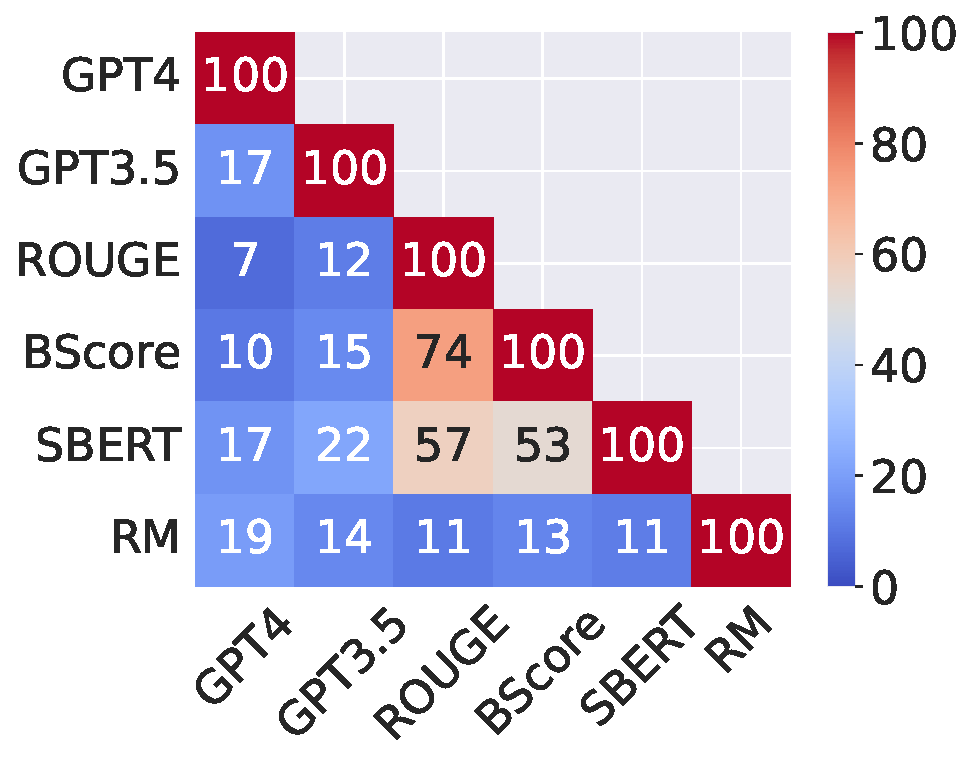
\includegraphics[width=\textwidth]{images/learning_dynamics/exp1a_corr.pdf}
    % \captionof{figure}{\textbf{Spearman $\rho$ between metrics} on synthetic data.}
    \label{fig:correlations}
    \end{minipage}
\end{figure*}
\subsection{Experimental setup}

\textbf{Training an IFT model.} IFT models are trained by fine-tuning a base model on a large instruction corpus, collected either through human annotations \sidecite{ouyang2022training, köpf2023openassistant} or concatenating task-specific datasets \sidecite{sanh2022multitask, mishra2022crosstask}. In line with recent work \sidecite{vicuna2023,wang2023selfinstruct,peng2023instruction}, we leverage synthetic data as the base instruction set in our IFT models \sidecite{alpaca2023}.
% Motivated by real-world industrial applications where cost is a primary concern, we rely on synthetic datasets to train the base IFT model.


\noindent\textbf{Benchmarking automatic metrics.} To benchmark the metrics, we rely on a combination of synthetic and real data.  For \emph{synthetic data}, we use the Alpaca GPT4 dataset \cite{alpaca2023}, and tag the data in 13 task categories (see \autoref{sec:alpaca-pres}) (\textit{e.g.}, logic, code, rewrite).  For \emph{human data}, we focus on tasks with industrial interests. Specifically, we include Natural Language Inference \sidecite{N18-1101, wang2019glue}, Question Answering \sidecite{rajpurkar2016squad}, NER \sidecite{tjong-kim-sang-de-meulder-2003-introduction}, and Sentiment Classification \sidecite{socher2013recursive, agirre-etal-2013-sem}). To build our metric evaluation dataset, we train and run LLaMA-7B models \cite{touvron2023llama} on varied data mixtures and target tasks. For rigor, we also report scores on the summarization with human feedback dataset from \sidecite{stiennon2022learning} (\texttt{SUM}).\sidenote{More details in \autoref{sec:exp_setup_1})}


\subsection{Experimental results}
To better understand the limitation of existing metrics we conduct both single-task analysis to ensure that metrics are able to score tasks reliably as well as multi-task analysis, which is the standard setting for IFT models. Results are reported in Tab. \ref{tab:main_metrics}.
% Insert table with checks or not

\noindent\textbf{\texttt{CIT} Analysis.} From Tab. \ref{tab:main_metrics}(left, \texttt{SUM}), we observe that the average correlation with human scores for evaluated summaries are higher for LLM models than with traditionally used metrics. Intra-task correlations on all other \emph{human data} tasks, averaged in \texttt{CIT} lead to similar conclusions. 


\noindent\textbf{\texttt{CAT} Analysis.} Tab. \ref{tab:main_metrics}(left) shows that all metrics, \emph{with the exception of the GPT4-based metric}, exhibit weak or no correlation in the context of inter-task consistency. While it is true that existing metrics demonstrate the ability to differentiate between good and bad samples within a single task (\texttt{CIT}), their \emph{performance falls short when confronted with the open setting imposed by IFT models}.
% here we could mention GPT3 bad results on CAT (see comment thread)
%u: très mal calibré sur de l inter taches, d autres scorers donnaient aussi des resultats negatifs ou nuls qu on a enlevé petit a petit, ca parait effectivement plus choquant mtn que les autres sont à ~20%il est aussi reference-free ce qui l handicappe intrinsequement sur des taches du genre, c est une conclusion qu on avaitmise a un moment, que le modele LLM de scoring se devait d etre bon en soit sur la tache en question pour avoir une chance


% Express 
\noindent\textbf{\texttt{TFA} Analysis.} On non-LLM-based metrics, performance gains reported between zero-shot models, and models trained on 1000 target-task samples (Tab. \ref{tab:main_metrics}(left), \texttt{TFA}) largely exceed the  12.0 \% relative improvement of human scores, and demonstrate how format, once learned, unrealistically boosts reference-based metrics which are heavily impacted by format.

\noindent\textbf{Metric Similarity Analysis.} \autoref{fig:correlations} displays metric correlation at the sample level on the synthetic dataset. The results align with \sidecite{chen2022reproducibility}, indicating a moderate to high correlation between BERT-based metrics and ROUGE-L. However, all metrics exhibit a low correlation with GPT4, indicating different response features are scored. 

\noindent\textbf{Zoom on GPT4.} Tab.\ref{tab:main_metrics}(right) shows a strong correlation between the results of GPT4-based metrics and the corresponding LLM task abilities reported in \sidecite{wei2022emergentabilitieslargelanguage} (Logic and Coding are non-trivial for LLMs, Writing tasks are relatively easier). However, reference-based metrics such as ROUGE suggest the opposite, as they are biased by the high syntactic overlap between model outputs and reference answers in these categories. The GPT3.5 scorer also highly rates results on the Logical Reasoning tasks, contrarily to GPT4. This is due to its lesser ability to spot logical inconsistencies in the evaluated responses \sidecite{bubeck2023sparks}, hinting that evaluator models must be capable at the evaluated task themselves in order to produce meaningful scores.

% \autoref{tab:main_metrics}(right) illustrates the importance of a unified scale across different tasks (as illustrated by automatically tagged classes such as logic, code, rewrite). We observe that the results of GPT4 correlate with related weaks and we found that some tasks (Logic) also require strong task abilities while task such as rewrite are easier. By considering other metrics such as ROUGE tge results is less clear (extract is harder that rewrite).


Our findings highlight the inadequacy of existing metrics in quantifying the performance of IFT models, while emphasizing GPT4 as a promising candidate. This performance gap in evaluation capabilities is primarily explained by GPT4's reduced dependence to reference answers, leading to a more coherent and absolute evaluation scale \texttt{CAT}, and an improved robustness to variations in output formatting \texttt{TFA}. \emph{The GPT4 scorer's powerful capabilities unlock the study of novel settings traditional metrics would struggle with} \sidecite{schaeffer2023emergent}.
% \emph{We find GPT4 to be a powerful scorer, unlocking the study of novel settings traditional metrics would struggle with.} \sidecite{schaeffer2023emergent}


\section{IFT Models for Industrial Applications}% Limits of evaluation metrics}
% \input{setup.tex}


\subsection{$\mathcal{S}_1$: Improving Specific Tasks}\label{ssec:scenario1}
In this section, we delve into $\mathcal{S}_1$, which specifically aims to extend an IFT model's capabilities to better perform on specific instructions.
%Motivated by industrial considerations, our goal is to assess the trade-off between data and quality in the performance of the final task.

%(i) How many samples are needed for a general-purpose model to "learn" a new task? (ii) Is learning an output format disentangled from improving the model's zero shot capacities on the task itself? (iii) Does learning a new task degrade the model's performance across other tasks?

\noindent\textbf{Setting.} We fine-tune a base 7B-LLM model (Pythia \sidecite{biderman2023pythia}, Bloom \sidecite{scao2022bloom}, Falcon \sidecite{penedo2023refinedweb}, or LLaMA) using synthetic instructions. In each training iteration, we introduce a selected number of $N$ \emph{real} target task samples into the synthetic dataset. We evaluate the model performance on an independent test subset of the target task. More experimental details are given in \autoref{sec:exp_setup_app_31}.
% These tasks are adapted from non-generative benchmarks and have been formatted to be processed by a generative LLM.
\begin{figure}[ht]
    \centering
    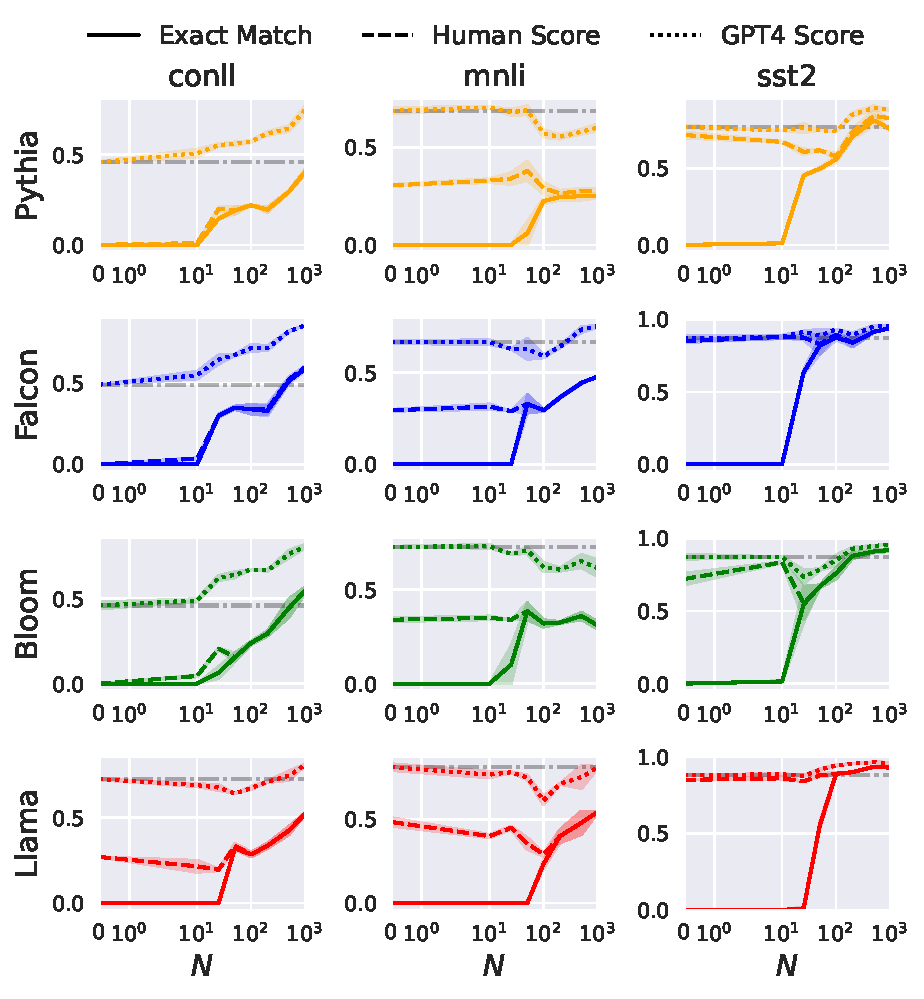
\includegraphics[width=0.8\textwidth]{images/learning_dynamics/exp1b_all.pdf}
    \caption[IFT training with real samples]{Incorporating $0 \leq N \leq 1000$ real task samples into IFT model training}
    \label{fig:exp1b_all}
\end{figure} %  N in \{10,50,100,200, 500,1000\}

\noindent\textbf{Mastering Format to Foster Understanding.} \autoref{fig:exp1b_all} shows target task performance as the number of target task samples introduced within the base training set increases. Across all tasks and models, \emph{specialization is biphasic}: first, \textit{task output format} is learned while overall performance remains constant, or even slightly decreases. Only once the format has been mastered, as noted by the spike of the Exact Match, does the model improve upon its \textit{underlying task performance} (Human and GPT4 scores increase), eventually surpassing the original zero-shot performance. It is worth noting that this analysis is made possible by format-agnostic scorers (\texttt{TFA}) that can accurately decouple output format from underlying model performance.

\noindent\textbf{Measuring Model Forgetting.} Performance on a test split of the Alpaca data shows little to no performance degradation (<1\%) caused by the inclusion of new tasks to the training mix (\autoref{sec:app_perf_deg}).


% \noindent \textbf{Harnessing Synthetic Datasets for Formatting Mastery} 
\noindent \textbf{Leveraging Synthetic Data to Learn to Format.} Our findings suggest a straightforward approach to optimizing the use of real examples: \emph{employ synthetic examples to assist the model in mastering the desired format before relying on real samples to enhance overall model performance}. We repeat the previous experiment, replacing the $N$  human-annotated target task training samples (\emph{H}), by GPT4 synthetically-generated samples  (\emph{S}), or synthetic samples with random labels (\emph{R}) (\autoref{fig:random}) \texttt{Exact Match} shows synthetic or randomly labeled data can indeed be used to learn the desired format, although the better quality human data eventually yields better results with more samples. In (\emph{S+H}), we train on 100 synthetic samples, then on $N$ human-annotated samples. This technique enables the model to master the format before being trained on high-quality data, largely improving human annotated data sample efficiency.
% However, comparable outcomes and more efficient learning can be attained by combining both \emph{synthetic} and \emph{human} datasets. As expected, clear performance degradation is seen in the Random setting past a certain number of samples.
%\emph{We can thus train our models to learn format on synthetic or low-quality data, to improve sample efficiency once training with real data !}

%A follow-up experiment displayed in Figure \ref{fig:random}, consists of replacing the target task by respectively a synthetic SST2-like dataset constructed from GPT4, and a variant of the latter in which positive/negative labels are given randomly. We see inherent task performance for the randomly labeled split only starts degrading after format is learned.



% Needs to be cleaned up
\begin{figure}[ht]
    \centering
    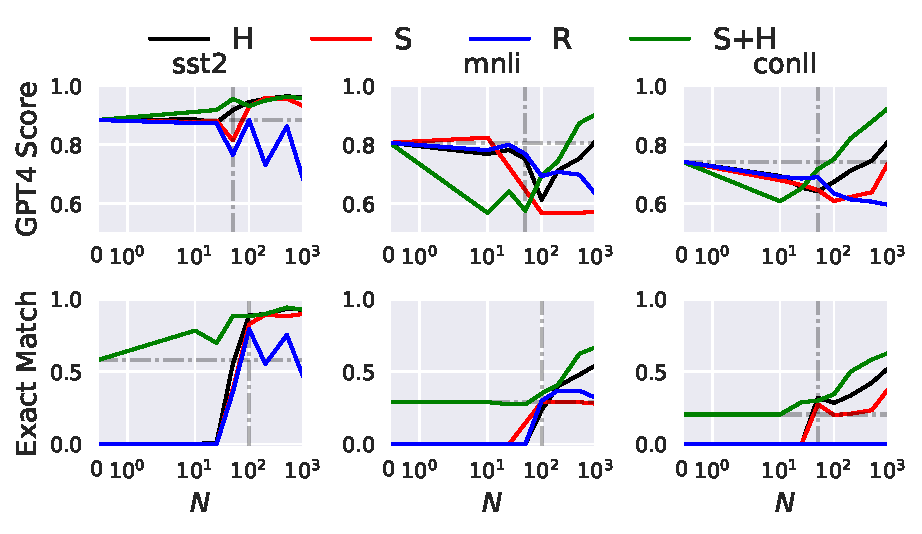
\includegraphics[width=0.8\textwidth]{images/learning_dynamics/sym_exp1.pdf}
    \caption[IFT training data mixes]{Incorporating  $0 \leq N \leq 1000$ (H)uman, (S)ynthetic and (R)andomly labeled synthetic data samples in IFT training set. (S+H) is trained on 100 synthetic samples, then $N$ human data samples. }\vspace{-.8cm}
    \label{fig:random}
\end{figure}



\subsection{$\mathcal{S}_2$: IFT models as Task-Specific Solvers}

%Motivated by industrial considerations, we delve into $\mathcal{S}_2$, which focuses on specializing IFT models on a specific task.

\noindent \textbf{Setting.} We use four model architectures and, for each architecture, we employ the base model to train an IFT model variant using the synthetic Alpaca dataset. We then fine-tune both the base models and their IFT variants on a subset of $N$ samples drawn from the target task. This setup simulates an industrial scenario in which limited data is available to specialize a model on a unique task, and assesses whether there are benefits to instruction-tuning a base model before fine-tuning it on the target task. 
\\\noindent \textbf{Results}. \autoref{fig:exp4} demonstrates that IFT models exhibit enhanced performance in low-data scenarios (when $10 \leq N \leq 200$). 
Intuitively, IFT models are better able to leverage the task description given in the prompts, thus enabling boosted zero-shot performance \sidecite{scao2021data}. This complements and steers model training when finetuned with small numbers of samples. When more samples are available ($N \geq 200$), the task pattern is sufficiently clear and the benefits of prompting and of the IFT training phase disappear.

 
\begin{figure}[ht]
    \centering
    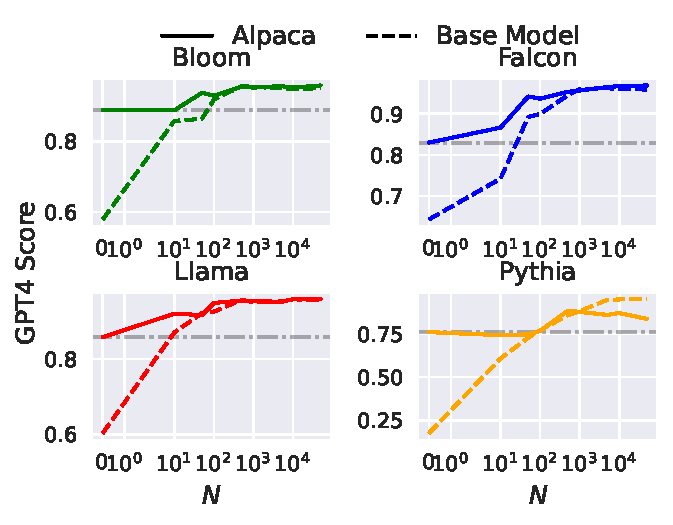
\includegraphics[width=0.8\textwidth]{images/learning_dynamics/exp4_all.pdf}
    \caption[GPT4 SST-2 scores]{GPT4 score on SST-2 test set after finetuning with $0 \leq N \leq 1000$  samples on a (base) LM or an IFT model. Further experiments can be found in \autoref{sec:extra-datasets-exp4}. }
    \label{fig:exp4}
\end{figure}

This finding aligns with the results presented in \autoref{ssec:scenario1}, emphasizing the potential of synthetic datasets to enhance data efficiency in industrial scenarios.


\section{Key Takeaways for Practitioners}
\label{sec:conclusion}

\noindent \textbf{Leveraging LLM for evaluation.} Evaluating IFT models is challenging, as it mandates \emph{comparability across tasks} and \emph{format-agnostism}, which standard metrics struggle with. While LLM scoring is not ideal (Limitations in \autoref{sec:limitations}), it is a strong option practitioners should add to their arsenal.
%consider in their evaluation strategy.
\\\noindent \textbf{Leveraging Synthetic Data for Efficient Learning.} LLM-based evaluation uncovers the fact that leveraging synthetic data provides a quick and cost-effective approach to mastering format in low data regimes, with no performance degradation. This methodology proves viable across various scenarios, presenting an opportunity to more efficiently leverage potentially limited amounts of expert annotated data available.
% significantly lower costs, which is particularly advantageous when incorporating expert annotations.



%Intuitively, including the target task in an IFT training set leads to better performance. However, performance improvements on a given task are only truly seen once the format is learned. Until then, performance tends to stay stable, or even decrease.
%\\\noindent Using an IFT model as the base model for fine-tuning offers large performance gains in very low shot training settings. Passed a certain number of shots, this benefit fully disappears.


% \section{Conclusion}
% 1 on highlight les limitations, le pb c'est qu'il n'y a que GPT4 (discusssed in limitation)
% 2 provide take-home lessons for practitionner and



%\setchapterpreamble[u]{\margintoc}

To do.

Mention prediction markets as a source of distributed information and as a benchmark and use case of search.



Tying back to the central theme of search, the conclusion outlines what the next generation of information access may look like. We argue that \emph{omnimodal} search will become central as the set of exploitable sources of information widens with model capabilites (text, images, audio, video, code, structured data, 3D models).
Recent projects such as BrowseComp illustrate the growing impact of AI agents on real-world information seeking and highlight that robust access to complex information benefits from \emph{adaptive compute}. Crucially, these systems still benefit from strong ``first-layer'' retrieval primitives such as embedding-based search for efficient candidate selection.

The conclusion further reflects on the fact that verifying search correctness is not uniformly easy. Instead, search exhibits a \emph{jagged frontier} of capabilities: some tasks (e.g., factual verification grounded in accessible digital sources) are comparatively straightforward to check and should steadily improve \sidenote{Although as demonstrated by Vidore V3, complex queries remain very lengthy to verify even for human experts.}, whereas underspecified requests, open-ended synthesis, and value-laden questions remain harder both to solve and to verify. In this lens, verifier-side constraints shape what kinds of search problems will be reliably improved ``verifier's law''. (Mention the fact a lot of weak signals are provided by the user in a tyoical search system and can be exploited to understand whether a system has satisified a user request (are they asking follow ups, etc).

We further note that not all information is equally accessible: some sources remain costly to reach, poorly indexed, private, ephemeral... Exploiting such information at scale will therefore remain challenging in the coming years. Looking forward, we anticipate a shift from explicit querying toward more \emph{implicit} information access, where systems proactively surface relevant knowledge continuously in response to context, goals, and ongoing activity.

Finally, we argue that long-context modeling and information retrieval are closer than they may appear, and that bridging these literatures can be fruitful: both fields study how to select, compress, and condition on relevant evidence, finding needles of relevamnt information in a haystack of noise. Building conceptual and methodological links between them may be possible.

Beyond the technical horizon, we close by reflecting on what truly frictionless information access would mean, and on the societal implications of delegating discovery, synthesis, and decision support to increasingly agentic systems.

% \subsection{Citations}

% We encourage you to use the natbib styles.
% You can use the command \verb|\sidecite| (cite in text) to get ``author (year)'' citations, like this citation to a paper by \sidecite{layoutlm}.
% You can use the command \verb|\sidecite| (cite in parentheses) to get ``(author, year)'' citations \sidecite{layoutlm}.
% You can use the command \verb|\citealp| (alternative cite without parentheses) to get ``author, year'' citations, which is useful for using citations within parentheses (e.g. \citealp{layoutlm}).

\section*{Limitations}
\label{sec:limitations}
While this paper has argued in favor of using LLM as scorers, important drawbacks remain. 
The best-performing scorer at the moment, GPT4 is a proprietary, black-box access model, and no guarantees exist that it will remain accessible unchanged over time, leading to reproducibility issues and data privacy concerns. Since model and training data internals are not open-knowledge, analysis of scoring errors and internal model biases is also limited. 

Promising openly available alternative models are being developed, either general purpose LLMs aiming to disrupt the hegemony of GPT4 \cite{touvron2023llama2, bai2023qwen}, or smaller models specialized for automatic evaluation, often attempting to distillate GPT4's scoring abilities by training on GPT4 generated scores or scoring explanations \sidecite{xu2023instructscore, liu2023geval}. In the latter category, the Prometheus scoring model \sidecite{kim2023prometheus}, based on Llama2, claims scoring performances on par with GPT4 in terms of human score correlations over a variety of tasks and benchmarks. Eventually, strong Open-Source LLMs should alleviate most of the concerns raised by relying on proprietary black-box models and we hope this work, by shedding light on the importance of LLM scoring, motivates these efforts to build open models with strong scoring abilities. 
% Pertaining to reproducibility, LLM scorers are sensitive to scoring prompt formulations. While not a problem in practice since the same prompt can be used across evaluations, some prompts are bound to be better than others, which will necessarily lead to various prompts being used across the literature, and hindering researcher ability to compare results against externally claimed baselines. 


% As seen in our experiments, to unlock truly good scoring, it is necessary for the scoring model to outperform evaluated models on the given task. While a large limitation of this scoring paradigm, weaker models can still evaluate better models on criteria they manage well, such as text coherence, relevance to the prompt, grammar, etc. even if the underlying task comprehension is not on-par. Work like INSTRUCTScore also show promising results of distilling GPT4 evaluation skills in smaller models like LLaMA 7B for specific tasks like translation.
% 


% ACL 2023 requires all submissions to have a section titled ``Limitations'', for discussing the limitations of the paper as a complement to the discussion of strengths in the main text. This section should occur after the conclusion, but before the references. It will not count towards the page limit. The discussion of limitations is mandatory. Papers without a limitation section will be desk-rejected without review.

% While we are open to different types of limitations, just mentioning that a set of results have been shown for English only probably does not reflect what we expect. Mentioning that the method works mostly for languages with limited morphology, like English, is a much better alternative. In addition, limitations such as low scalability to long text, the requirement of large GPU resources, or other things that inspire crucial further investigation are welcome.

\section*{Ethics Statement}
% Scientific work published at ACL 2023 must comply with the ACL Ethics Policy.\sidenote{\url{https://www.aclweb.org/portal/content/acl-code-ethics}} We encourage all authors to include an explicit ethics statement on the broader impact of the work, or other ethical considerations after the conclusion but before the references. The ethics statement will not count toward the page limit (8 pages for long, 4 pages for short papers).

While this work intends to evaluate scorers across many different tasks and settings, it is essentially English-centric, and no conclusions are drawn about the robustness of LLM scorers in other languages. LLM scoring may also be affected by internal model bias acquired through pretraining or subsequent finetuning, and while efforts are made by OpenAI to mitigate bias, critical applications of LLM evaluation should consider that truly objective evaluation is not attainable.

All data and base models used in this work originate from publicly available sources. The GPT4 Alpaca dataset is a variant of \sidecite{alpaca2023} built from synthetic data only, collected through the OpenAI API. The non-synthetic data are sourced from manually annotated, widely used datasets for NLP benchmarking. This work does not transgress any usage restrictions associated with these data sources. Base models used are either available through fully open-source licenses (Falcon, Pythia), or licenses with no restrictions for research purposes (LLaMA, Bloom). 

We estimate our experiments consumed 5500 GPU V100 hours, using a low-carbon compute cluster, amounting to about 950 kg of CO2 over the course of the project.  To reduce the impact to a maximum, all runs are done through the efficient Low-Rank Adaptation training strategy \sidecite{hu2021loralowrankadaptationlarge}, and only trained adapter weights are stored to minimize bandwidth and memory usage. API calls to external APIs are cached to minimize redundancies.


\section*{Acknowledgements}
This work is partially supported by Illuin Technology, and by a grant from ANRT France.
This work was performed using HPC resources from GENCI–IDRIS (Grant 2023-AD011014185).
Secondary compute contributions were made on HPC resources (Grant 2023-AD103256) and (Grant 2023-AD101838).
